% **************************************************************************************************************
% A Classic Thesis Style
% An Homage to The Elements of Typographic Style
%
% Copyright (C) 2015 André Miede http://www.miede.de
%
% If you like the style then I would appreciate a postcard. My address 
% can be found in the file ClassicThesis.pdf. A collection of the 
% postcards I received so far is available online at 
% http://postcards.miede.de
%
% License:
% This program is free software; you can redistribute it and/or modify
% it under the terms of the GNU General Public License as published by
% the Free Software Foundation; either version 2 of the License, or
% (at your option) any later version.
%
% This program is distributed in the hope that it will be useful,
% but WITHOUT ANY WARRANTY; without even the implied warranty of
% MERCHANTABILITY or FITNESS FOR A PARTICULAR PURPOSE.  See the
% GNU General Public License for more details.
%
% You should have received a copy of the GNU General Public License
% along with this program; see the file COPYING.  If not, write to
% the Free Software Foundation, Inc., 59 Temple Place - Suite 330,
% Boston, MA 02111-1307, USA.
%
% **************************************************************************************************************
\RequirePackage{fix-cm} % fix some latex issues see: http://texdoc.net/texmf-dist/doc/latex/base/fixltx2e.pdf
\documentclass[ twoside,openright,titlepage,numbers=noenddot,headinclude,%1headlines,% letterpaper a4paper
                footinclude=true,cleardoublepage=empty,abstractoff, % <--- obsolete, remove (todo)
                BCOR=5mm,paper=a4,fontsize=11pt,%11pt,a4paper,%
                ngerman,american,%
                ]{scrreprt}

% ****************************************************************************************************
% Set the encoding of your files. UTF-8 is the only sensible encoding nowadays. If you can't read
% äöüßáéçèê∂åëæƒÏ€ then change the encoding setting in your editor, not the line below. If your editor
% does not support utf8 use another editor!
% ****************************************************************************************************
\PassOptionsToPackage{utf8}{inputenc}
	\usepackage{inputenc}
	
\usepackage{etoolbox}

% ****************************************************************************************************
% Insert the information about your thesis here
% ****************************************************************************************************
\newcommand{\myTitle}{AnSiAn - Android Signal Analyzer\xspace}
\newcommand{\myDegree}{Secure Mobile Networking Project Documentation\xspace}
\newcommand{\myName}{Matthias Kannwischer\xspace}
\newcommand{\myProf}{Prof. Dr.-Ing. Matthias Hollick\xspace}
%\newcommand{\myOtherProf}{Second advisor\xspace}
\newcommand{\mySupervisor}{Jiska Classen\xspace}
\newcommand{\myFaculty}{Department of Computer Science\xspace}
\newcommand{\myDepartment}{Secure Mobile Networking Lab\xspace}
\newcommand{\myUni}{\protect{Technische Universität Darmstadt}\xspace}
\newcommand{\myLocation}{Darmstadt\xspace}
\newcommand{\myTime}{\formatdate{09}{03}{2017}\xspace}
\newcommand{\myVersion}{0.1\xspace}

% Choose if you want the standard template with enough space for margin notes or the tempate with small margins
\newtoggle{adrianstyle}
%\toggletrue{adrianstyle} % uncomment this line to have smaller margins
\togglefalse{adrianstyle} % uncomment this line for the standard seemoo template

%********************************************************************
% Note: Make all your adjustments in here
%*******************************************************
% ****************************************************************************************************
% classicthesis-config.tex 
% formerly known as loadpackages.sty, classicthesis-ldpkg.sty, and classicthesis-preamble.sty 
% Use it at the beginning of your ClassicThesis.tex, or as a LaTeX Preamble 
% in your ClassicThesis.{tex,lyx} with % ****************************************************************************************************
% classicthesis-config.tex 
% formerly known as loadpackages.sty, classicthesis-ldpkg.sty, and classicthesis-preamble.sty 
% Use it at the beginning of your ClassicThesis.tex, or as a LaTeX Preamble 
% in your ClassicThesis.{tex,lyx} with % ****************************************************************************************************
% classicthesis-config.tex 
% formerly known as loadpackages.sty, classicthesis-ldpkg.sty, and classicthesis-preamble.sty 
% Use it at the beginning of your ClassicThesis.tex, or as a LaTeX Preamble 
% in your ClassicThesis.{tex,lyx} with \input{classicthesis-config}
% ****************************************************************************************************  
% If you like the classicthesis, then I would appreciate a postcard. 
% My address can be found in the file ClassicThesis.pdf. A collection 
% of the postcards I received so far is available online at 
% http://postcards.miede.de
% ****************************************************************************************************

% ****************************************************************************************************
% 1. Configure classicthesis for your needs here, e.g., remove "drafting" below 
% in order to deactivate the time-stamp on the pages
% ****************************************************************************************************
\PassOptionsToPackage{eulerchapternumbers,listings,%
                 %drafting,%
				 pdfspacing,%floatperchapter,%linedheaders,%
				 subfig,beramono,eulermath,parts,dottedtoc,%
				 \iftoggle{adrianstyle}{adrianstyle}{}, % Use this option to increase the text width
				 }{classicthesis}								
% ********************************************************************
% Available options for classicthesis.sty 
% (see ClassicThesis.pdf for more information):
% drafting
% parts nochapters linedheaders
% eulerchapternumbers beramono eulermath pdfspacing minionprospacing
% tocaligned dottedtoc manychapters
% listings floatperchapter subfig
% ********************************************************************


% ****************************************************************************************************
% 2. Loading some handy packages
% ****************************************************************************************************
%\PassOptionsToPackage{spanish,es-lcroman}{babel}

% ********************************************************************
% Setup, finetuning, and useful commands
% ********************************************************************
\newcounter{dummy} % necessary for correct hyperlinks (to index, bib, etc.)
\newlength{\abcd} % for ab..z string length calculation
% ****************************************************************************************************


% ****************************************************************************************************
% 3. Loading some handy packages
% ****************************************************************************************************
% ******************************************************************** 
% Packages with options that might require adjustments
% ******************************************************************** 
%\PassOptionsToPackage{ngerman,american}{babel}   % change this to your language(s)
% Spanish languages need extra options in order to work with this template
%\PassOptionsToPackage{spanish,es-lcroman}{babel}
	\usepackage{babel}                  

\usepackage{csquotes}
\PassOptionsToPackage{%
    %backend=biber, %instead of bibtex
	backend=bibtex8,bibencoding=ascii,%
	language=auto,%
	style=numeric-comp,%
    %style=authoryear-comp, % Author 1999, 2010
    %bibstyle=authoryear,dashed=false, % dashed: substitute rep. author with ---
    sorting=nyt, % name, year, title
    maxbibnames=10, % default: 3, et al.
    %backref=true,%
    natbib=true % natbib compatibility mode (\citep and \citet still work)
}{biblatex}
    \usepackage{biblatex}

\PassOptionsToPackage{fleqn}{amsmath}       % math environments and more by the AMS 
    \usepackage{amsmath}

% ******************************************************************** 
% General useful packages
% ******************************************************************** 
\PassOptionsToPackage{T1}{fontenc} % T2A for cyrillics
    \usepackage{fontenc}     
\usepackage{textcomp} % fix warning with missing font shapes
\usepackage{scrhack} % fix warnings when using KOMA with listings package          
\usepackage{xspace} % to get the spacing after macros right  
\usepackage{mparhack} % get marginpar right
\usepackage{fixltx2e} % fixes some LaTeX stuff --> since 2015 in the LaTeX kernel (see below)
\usepackage{acronym}
%\usepackage[latest]{latexrelease} % will be used once available in more distributions (ISSUE #107)
%\usepackage[nopostdot,acronym,shortcuts,nonumberlist]{glossaries}
%\makeglossaries
%\renewcommand*{\glossarysection}[2][]{}
%\input{acronyms.tex}

% ****************************************************************************************************


% ****************************************************************************************************
% 4. Setup floats: tables, (sub)figures, and captions
% ****************************************************************************************************
\usepackage{tabularx} % better tables
    \setlength{\extrarowheight}{3pt} % increase table row height
\newcommand{\tableheadline}[1]{\multicolumn{1}{c}{\spacedlowsmallcaps{#1}}}
\newcommand{\myfloatalign}{\centering} % to be used with each float for alignment
\usepackage{caption}
% Thanks to cgnieder and Claus Lahiri
% http://tex.stackexchange.com/questions/69349/spacedlowsmallcaps-in-caption-label
% [REMOVED DUE TO OTHER PROBLEMS, SEE ISSUE #82]    
%\DeclareCaptionLabelFormat{smallcaps}{\bothIfFirst{#1}{~}\MakeTextLowercase{\textsc{#2}}}
%\captionsetup{font=small,labelformat=smallcaps} % format=hang,
\captionsetup{font=small} % format=hang,
\usepackage{subfig}  
% ****************************************************************************************************


% ****************************************************************************************************
% 5. Setup code listings
% ****************************************************************************************************
\usepackage{listings} 
%\lstset{emph={trueIndex,root},emphstyle=\color{BlueViolet}}%\underbar} % for special keywords
\lstset{language=[LaTeX]Tex,%C++,
    morekeywords={PassOptionsToPackage,selectlanguage},
    keywordstyle=\color{RoyalBlue},%\bfseries,
    basicstyle=\small\ttfamily,
    %identifierstyle=\color{NavyBlue},
    commentstyle=\color{Green}\ttfamily,
    stringstyle=\rmfamily,
    numbers=none,%left,%
    numberstyle=\scriptsize,%\tiny
    stepnumber=5,
    numbersep=8pt,
    showstringspaces=false,
    breaklines=true,
    %frameround=ftff,
    %frame=single,
    belowcaptionskip=.75\baselineskip
    %frame=L
} 
% ****************************************************************************************************    		   


% ****************************************************************************************************
% 6. PDFLaTeX, hyperreferences and citation backreferences
% ****************************************************************************************************
% ********************************************************************
% Using PDFLaTeX
% ********************************************************************
\PassOptionsToPackage{pdftex,hyperfootnotes=false,pdfpagelabels}{hyperref}
    \usepackage{hyperref}  % backref linktocpage pagebackref
\pdfcompresslevel=9
\pdfadjustspacing=1 
\PassOptionsToPackage{pdftex}{graphicx}
    \usepackage{graphicx} 
 

% ********************************************************************
% Hyperreferences
% ********************************************************************
\hypersetup{%
    %draft,	% = no hyperlinking at all (useful in b/w printouts)
    %colorlinks=true, linktocpage=true, pdfstartpage=3, pdfstartview=FitV,%
    % uncomment the following line if you want to have black links (e.g., for printing)
    colorlinks=false, linktocpage=false, pdfborder={0 0 0}, pdfstartpage=3, pdfstartview=FitV,% 
    breaklinks=true, pdfpagemode=UseNone, pageanchor=true, pdfpagemode=UseOutlines,%
    plainpages=false, bookmarksnumbered, bookmarksopen=true, bookmarksopenlevel=1,%
    hypertexnames=true, pdfhighlight=/O,%nesting=true,%frenchlinks,%
    urlcolor=webbrown, linkcolor=RoyalBlue, citecolor=webgreen, %pagecolor=RoyalBlue,%
    %urlcolor=Black, linkcolor=Black, citecolor=Black, %pagecolor=Black,%
    pdftitle={\myTitle},%
    pdfauthor={\textcopyright\ \myName, \myUni, \myFaculty},%
    pdfsubject={},%
    pdfkeywords={},%
    pdfcreator={pdfLaTeX},%
    pdfproducer={LaTeX with hyperref and classicthesis}%
}

\pdfinfo{
   /CreationDate (D:20130424083342)
   /ModDate (D:20130424083342)
}

% ********************************************************************
% Setup autoreferences
% ********************************************************************
% There are some issues regarding autorefnames
% http://www.ureader.de/msg/136221647.aspx
% http://www.tex.ac.uk/cgi-bin/texfaq2html?label=latexwords
% you have to redefine the makros for the 
% language you use, e.g., american, ngerman
% (as chosen when loading babel/AtBeginDocument)
% ********************************************************************
\makeatletter
\@ifpackageloaded{babel}%
    {%
       \addto\extrasamerican{%
			\renewcommand*{\figureautorefname}{Figure}%
			\renewcommand*{\tableautorefname}{Table}%
			\renewcommand*{\partautorefname}{Part}%
			\renewcommand*{\chapterautorefname}{Chapter}%
			\renewcommand*{\sectionautorefname}{Section}%
			\renewcommand*{\subsectionautorefname}{Section}%
			\renewcommand*{\subsubsectionautorefname}{Section}%     
                }%
       \addto\extrasngerman{% 
			\renewcommand*{\paragraphautorefname}{Absatz}%
			\renewcommand*{\subparagraphautorefname}{Unterabsatz}%
			\renewcommand*{\footnoteautorefname}{Fu\"snote}%
			\renewcommand*{\FancyVerbLineautorefname}{Zeile}%
			\renewcommand*{\theoremautorefname}{Theorem}%
			\renewcommand*{\appendixautorefname}{Anhang}%
			\renewcommand*{\equationautorefname}{Gleichung}%        
			\renewcommand*{\itemautorefname}{Punkt}%
                }%  
            % Fix to getting autorefs for subfigures right (thanks to Belinda Vogt for changing the definition)
            \providecommand{\subfigureautorefname}{\figureautorefname}%             
    }{\relax}
\makeatother


% ****************************************************************************************************
% 7. Last calls before the bar closes
% ****************************************************************************************************
% ********************************************************************
% Development Stuff
% ********************************************************************
\listfiles
%\PassOptionsToPackage{l2tabu,orthodox,abort}{nag}
%   \usepackage{nag}
%\PassOptionsToPackage{warning, all}{onlyamsmath}
%   \usepackage{onlyamsmath}

% ********************************************************************
% Last, but not least...
% ********************************************************************
\usepackage{classicthesis} 
% ****************************************************************************************************


% ****************************************************************************************************
% 8. Further adjustments (experimental)
% ****************************************************************************************************
% ********************************************************************
% Changing the text area
% ********************************************************************
%\linespread{1.05} % a bit more for Palatino
%\areaset[current]{312pt}{761pt} % 686 (factor 2.2) + 33 head + 42 head \the\footskip
%\setlength{\marginparwidth}{7em}%
%\setlength{\marginparsep}{2em}%

% ********************************************************************
% Using different fonts
% ********************************************************************
%\usepackage[oldstylenums]{kpfonts} % oldstyle notextcomp
%\usepackage[osf]{libertine}
%\usepackage[light,condensed,math]{iwona}
%\renewcommand{\sfdefault}{iwona}
%\usepackage{lmodern} % <-- no osf support :-(
%\usepackage{cfr-lm} % 
%\usepackage[urw-garamond]{mathdesign} <-- no osf support :-(
%\usepackage[default,osfigures]{opensans} % scale=0.95 
%\usepackage[sfdefault]{FiraSans}
% ****************************************************************************************************

% ****************************************************************************************************  
% If you like the classicthesis, then I would appreciate a postcard. 
% My address can be found in the file ClassicThesis.pdf. A collection 
% of the postcards I received so far is available online at 
% http://postcards.miede.de
% ****************************************************************************************************

% ****************************************************************************************************
% 1. Configure classicthesis for your needs here, e.g., remove "drafting" below 
% in order to deactivate the time-stamp on the pages
% ****************************************************************************************************
\PassOptionsToPackage{eulerchapternumbers,listings,%
                 %drafting,%
				 pdfspacing,%floatperchapter,%linedheaders,%
				 subfig,beramono,eulermath,parts,dottedtoc,%
				 \iftoggle{adrianstyle}{adrianstyle}{}, % Use this option to increase the text width
				 }{classicthesis}								
% ********************************************************************
% Available options for classicthesis.sty 
% (see ClassicThesis.pdf for more information):
% drafting
% parts nochapters linedheaders
% eulerchapternumbers beramono eulermath pdfspacing minionprospacing
% tocaligned dottedtoc manychapters
% listings floatperchapter subfig
% ********************************************************************


% ****************************************************************************************************
% 2. Loading some handy packages
% ****************************************************************************************************
%\PassOptionsToPackage{spanish,es-lcroman}{babel}

% ********************************************************************
% Setup, finetuning, and useful commands
% ********************************************************************
\newcounter{dummy} % necessary for correct hyperlinks (to index, bib, etc.)
\newlength{\abcd} % for ab..z string length calculation
% ****************************************************************************************************


% ****************************************************************************************************
% 3. Loading some handy packages
% ****************************************************************************************************
% ******************************************************************** 
% Packages with options that might require adjustments
% ******************************************************************** 
%\PassOptionsToPackage{ngerman,american}{babel}   % change this to your language(s)
% Spanish languages need extra options in order to work with this template
%\PassOptionsToPackage{spanish,es-lcroman}{babel}
	\usepackage{babel}                  

\usepackage{csquotes}
\PassOptionsToPackage{%
    %backend=biber, %instead of bibtex
	backend=bibtex8,bibencoding=ascii,%
	language=auto,%
	style=numeric-comp,%
    %style=authoryear-comp, % Author 1999, 2010
    %bibstyle=authoryear,dashed=false, % dashed: substitute rep. author with ---
    sorting=nyt, % name, year, title
    maxbibnames=10, % default: 3, et al.
    %backref=true,%
    natbib=true % natbib compatibility mode (\citep and \citet still work)
}{biblatex}
    \usepackage{biblatex}

\PassOptionsToPackage{fleqn}{amsmath}       % math environments and more by the AMS 
    \usepackage{amsmath}

% ******************************************************************** 
% General useful packages
% ******************************************************************** 
\PassOptionsToPackage{T1}{fontenc} % T2A for cyrillics
    \usepackage{fontenc}     
\usepackage{textcomp} % fix warning with missing font shapes
\usepackage{scrhack} % fix warnings when using KOMA with listings package          
\usepackage{xspace} % to get the spacing after macros right  
\usepackage{mparhack} % get marginpar right
\usepackage{fixltx2e} % fixes some LaTeX stuff --> since 2015 in the LaTeX kernel (see below)
\usepackage{acronym}
%\usepackage[latest]{latexrelease} % will be used once available in more distributions (ISSUE #107)
%\usepackage[nopostdot,acronym,shortcuts,nonumberlist]{glossaries}
%\makeglossaries
%\renewcommand*{\glossarysection}[2][]{}
%\newacronym{NIC}{NIC}{network interface card}
\newacronym{EMR}{EMR}{electromagnetic radiation}
\newacronym{NSA}{NSA}{National Security Agency}
\newacronym{PC}{PC}{personal computer}
\newacronym{USRP}{USRP}{Universal Software Radio Peripheral}
\newacronym{SDR}{SDR}{software-defined radio}
\newacronym{FPGA}{FPGA}{field-programmable gate array}
\newacronym{PA}{PA}{power amplifier}
\newacronym{BCI}{BCI}{bulk current injection}
\newacronym{FEC}{FEC}{forward error correction}
\newacronym{IEC}{IEC}{International Electrotechnical Commission}
\newacronym{SFD}{SFD}{start frame delimiter}
\newacronym{MAC}{MAC}{Medium Access Control}
\newacronym{DAC}{DAC}{digital-to-analog converter}
\newacronym{CSMACD}{CSMA/CD}{carrier sense multiple access with collision detection}
\newacronym{CAN}{CAN}{control area network}
\newacronym{CoE}{CoE}{CAN over Ethernet}
\newacronym{RF}{RF}{radio frequency}
\newacronym{FCS}{FCS}{frame check sum}
\newacronym{ADC}{ADC}{analog-to-digital converter}
\newacronym{(S+N)/NR}{(S+N)/NR}{signal-plus-noise-to-noise ratio}
\newacronym{ICMP}{ICMP}{Internet control message protocol}
\newacronym{DoS}{DoS}{denial of service}
\newacronym{CRT}{CRT}{cathode ray tube}
\newacronym{SNR}{SNR}{signal-to-noise ratio}

\newacronym{AnSiAn}{AnSiAn}{Android Signal Analyzer}
\newacronym{RDS}{RDS}{Radio Data System}
\newacronym{BPSK}{BPSK}{Binary Phase Shift Keying}
\newacronym{QAM}{QAM}{Quadrature amplitude modulation}
\newacronym{FM}{FM}{Frequency Modulation}

% ****************************************************************************************************


% ****************************************************************************************************
% 4. Setup floats: tables, (sub)figures, and captions
% ****************************************************************************************************
\usepackage{tabularx} % better tables
    \setlength{\extrarowheight}{3pt} % increase table row height
\newcommand{\tableheadline}[1]{\multicolumn{1}{c}{\spacedlowsmallcaps{#1}}}
\newcommand{\myfloatalign}{\centering} % to be used with each float for alignment
\usepackage{caption}
% Thanks to cgnieder and Claus Lahiri
% http://tex.stackexchange.com/questions/69349/spacedlowsmallcaps-in-caption-label
% [REMOVED DUE TO OTHER PROBLEMS, SEE ISSUE #82]    
%\DeclareCaptionLabelFormat{smallcaps}{\bothIfFirst{#1}{~}\MakeTextLowercase{\textsc{#2}}}
%\captionsetup{font=small,labelformat=smallcaps} % format=hang,
\captionsetup{font=small} % format=hang,
\usepackage{subfig}  
% ****************************************************************************************************


% ****************************************************************************************************
% 5. Setup code listings
% ****************************************************************************************************
\usepackage{listings} 
%\lstset{emph={trueIndex,root},emphstyle=\color{BlueViolet}}%\underbar} % for special keywords
\lstset{language=[LaTeX]Tex,%C++,
    morekeywords={PassOptionsToPackage,selectlanguage},
    keywordstyle=\color{RoyalBlue},%\bfseries,
    basicstyle=\small\ttfamily,
    %identifierstyle=\color{NavyBlue},
    commentstyle=\color{Green}\ttfamily,
    stringstyle=\rmfamily,
    numbers=none,%left,%
    numberstyle=\scriptsize,%\tiny
    stepnumber=5,
    numbersep=8pt,
    showstringspaces=false,
    breaklines=true,
    %frameround=ftff,
    %frame=single,
    belowcaptionskip=.75\baselineskip
    %frame=L
} 
% ****************************************************************************************************    		   


% ****************************************************************************************************
% 6. PDFLaTeX, hyperreferences and citation backreferences
% ****************************************************************************************************
% ********************************************************************
% Using PDFLaTeX
% ********************************************************************
\PassOptionsToPackage{pdftex,hyperfootnotes=false,pdfpagelabels}{hyperref}
    \usepackage{hyperref}  % backref linktocpage pagebackref
\pdfcompresslevel=9
\pdfadjustspacing=1 
\PassOptionsToPackage{pdftex}{graphicx}
    \usepackage{graphicx} 
 

% ********************************************************************
% Hyperreferences
% ********************************************************************
\hypersetup{%
    %draft,	% = no hyperlinking at all (useful in b/w printouts)
    %colorlinks=true, linktocpage=true, pdfstartpage=3, pdfstartview=FitV,%
    % uncomment the following line if you want to have black links (e.g., for printing)
    colorlinks=false, linktocpage=false, pdfborder={0 0 0}, pdfstartpage=3, pdfstartview=FitV,% 
    breaklinks=true, pdfpagemode=UseNone, pageanchor=true, pdfpagemode=UseOutlines,%
    plainpages=false, bookmarksnumbered, bookmarksopen=true, bookmarksopenlevel=1,%
    hypertexnames=true, pdfhighlight=/O,%nesting=true,%frenchlinks,%
    urlcolor=webbrown, linkcolor=RoyalBlue, citecolor=webgreen, %pagecolor=RoyalBlue,%
    %urlcolor=Black, linkcolor=Black, citecolor=Black, %pagecolor=Black,%
    pdftitle={\myTitle},%
    pdfauthor={\textcopyright\ \myName, \myUni, \myFaculty},%
    pdfsubject={},%
    pdfkeywords={},%
    pdfcreator={pdfLaTeX},%
    pdfproducer={LaTeX with hyperref and classicthesis}%
}

\pdfinfo{
   /CreationDate (D:20130424083342)
   /ModDate (D:20130424083342)
}

% ********************************************************************
% Setup autoreferences
% ********************************************************************
% There are some issues regarding autorefnames
% http://www.ureader.de/msg/136221647.aspx
% http://www.tex.ac.uk/cgi-bin/texfaq2html?label=latexwords
% you have to redefine the makros for the 
% language you use, e.g., american, ngerman
% (as chosen when loading babel/AtBeginDocument)
% ********************************************************************
\makeatletter
\@ifpackageloaded{babel}%
    {%
       \addto\extrasamerican{%
			\renewcommand*{\figureautorefname}{Figure}%
			\renewcommand*{\tableautorefname}{Table}%
			\renewcommand*{\partautorefname}{Part}%
			\renewcommand*{\chapterautorefname}{Chapter}%
			\renewcommand*{\sectionautorefname}{Section}%
			\renewcommand*{\subsectionautorefname}{Section}%
			\renewcommand*{\subsubsectionautorefname}{Section}%     
                }%
       \addto\extrasngerman{% 
			\renewcommand*{\paragraphautorefname}{Absatz}%
			\renewcommand*{\subparagraphautorefname}{Unterabsatz}%
			\renewcommand*{\footnoteautorefname}{Fu\"snote}%
			\renewcommand*{\FancyVerbLineautorefname}{Zeile}%
			\renewcommand*{\theoremautorefname}{Theorem}%
			\renewcommand*{\appendixautorefname}{Anhang}%
			\renewcommand*{\equationautorefname}{Gleichung}%        
			\renewcommand*{\itemautorefname}{Punkt}%
                }%  
            % Fix to getting autorefs for subfigures right (thanks to Belinda Vogt for changing the definition)
            \providecommand{\subfigureautorefname}{\figureautorefname}%             
    }{\relax}
\makeatother


% ****************************************************************************************************
% 7. Last calls before the bar closes
% ****************************************************************************************************
% ********************************************************************
% Development Stuff
% ********************************************************************
\listfiles
%\PassOptionsToPackage{l2tabu,orthodox,abort}{nag}
%   \usepackage{nag}
%\PassOptionsToPackage{warning, all}{onlyamsmath}
%   \usepackage{onlyamsmath}

% ********************************************************************
% Last, but not least...
% ********************************************************************
\usepackage{classicthesis} 
% ****************************************************************************************************


% ****************************************************************************************************
% 8. Further adjustments (experimental)
% ****************************************************************************************************
% ********************************************************************
% Changing the text area
% ********************************************************************
%\linespread{1.05} % a bit more for Palatino
%\areaset[current]{312pt}{761pt} % 686 (factor 2.2) + 33 head + 42 head \the\footskip
%\setlength{\marginparwidth}{7em}%
%\setlength{\marginparsep}{2em}%

% ********************************************************************
% Using different fonts
% ********************************************************************
%\usepackage[oldstylenums]{kpfonts} % oldstyle notextcomp
%\usepackage[osf]{libertine}
%\usepackage[light,condensed,math]{iwona}
%\renewcommand{\sfdefault}{iwona}
%\usepackage{lmodern} % <-- no osf support :-(
%\usepackage{cfr-lm} % 
%\usepackage[urw-garamond]{mathdesign} <-- no osf support :-(
%\usepackage[default,osfigures]{opensans} % scale=0.95 
%\usepackage[sfdefault]{FiraSans}
% ****************************************************************************************************

% ****************************************************************************************************  
% If you like the classicthesis, then I would appreciate a postcard. 
% My address can be found in the file ClassicThesis.pdf. A collection 
% of the postcards I received so far is available online at 
% http://postcards.miede.de
% ****************************************************************************************************

% ****************************************************************************************************
% 1. Configure classicthesis for your needs here, e.g., remove "drafting" below 
% in order to deactivate the time-stamp on the pages
% ****************************************************************************************************
\PassOptionsToPackage{eulerchapternumbers,listings,%
                 %drafting,%
				 pdfspacing,%floatperchapter,%linedheaders,%
				 subfig,beramono,eulermath,parts,dottedtoc,%
				 \iftoggle{adrianstyle}{adrianstyle}{}, % Use this option to increase the text width
				 }{classicthesis}								
% ********************************************************************
% Available options for classicthesis.sty 
% (see ClassicThesis.pdf for more information):
% drafting
% parts nochapters linedheaders
% eulerchapternumbers beramono eulermath pdfspacing minionprospacing
% tocaligned dottedtoc manychapters
% listings floatperchapter subfig
% ********************************************************************


% ****************************************************************************************************
% 2. Loading some handy packages
% ****************************************************************************************************
%\PassOptionsToPackage{spanish,es-lcroman}{babel}

% ********************************************************************
% Setup, finetuning, and useful commands
% ********************************************************************
\newcounter{dummy} % necessary for correct hyperlinks (to index, bib, etc.)
\newlength{\abcd} % for ab..z string length calculation
% ****************************************************************************************************


% ****************************************************************************************************
% 3. Loading some handy packages
% ****************************************************************************************************
% ******************************************************************** 
% Packages with options that might require adjustments
% ******************************************************************** 
%\PassOptionsToPackage{ngerman,american}{babel}   % change this to your language(s)
% Spanish languages need extra options in order to work with this template
%\PassOptionsToPackage{spanish,es-lcroman}{babel}
	\usepackage{babel}                  

\usepackage{csquotes}
\PassOptionsToPackage{%
    %backend=biber, %instead of bibtex
	backend=bibtex8,bibencoding=ascii,%
	language=auto,%
	style=numeric-comp,%
    %style=authoryear-comp, % Author 1999, 2010
    %bibstyle=authoryear,dashed=false, % dashed: substitute rep. author with ---
    sorting=nyt, % name, year, title
    maxbibnames=10, % default: 3, et al.
    %backref=true,%
    natbib=true % natbib compatibility mode (\citep and \citet still work)
}{biblatex}
    \usepackage{biblatex}

\PassOptionsToPackage{fleqn}{amsmath}       % math environments and more by the AMS 
    \usepackage{amsmath}

% ******************************************************************** 
% General useful packages
% ******************************************************************** 
\PassOptionsToPackage{T1}{fontenc} % T2A for cyrillics
    \usepackage{fontenc}     
\usepackage{textcomp} % fix warning with missing font shapes
\usepackage{scrhack} % fix warnings when using KOMA with listings package          
\usepackage{xspace} % to get the spacing after macros right  
\usepackage{mparhack} % get marginpar right
\usepackage{fixltx2e} % fixes some LaTeX stuff --> since 2015 in the LaTeX kernel (see below)
\usepackage{acronym}
%\usepackage[latest]{latexrelease} % will be used once available in more distributions (ISSUE #107)
%\usepackage[nopostdot,acronym,shortcuts,nonumberlist]{glossaries}
%\makeglossaries
%\renewcommand*{\glossarysection}[2][]{}
%\newacronym{NIC}{NIC}{network interface card}
\newacronym{EMR}{EMR}{electromagnetic radiation}
\newacronym{NSA}{NSA}{National Security Agency}
\newacronym{PC}{PC}{personal computer}
\newacronym{USRP}{USRP}{Universal Software Radio Peripheral}
\newacronym{SDR}{SDR}{software-defined radio}
\newacronym{FPGA}{FPGA}{field-programmable gate array}
\newacronym{PA}{PA}{power amplifier}
\newacronym{BCI}{BCI}{bulk current injection}
\newacronym{FEC}{FEC}{forward error correction}
\newacronym{IEC}{IEC}{International Electrotechnical Commission}
\newacronym{SFD}{SFD}{start frame delimiter}
\newacronym{MAC}{MAC}{Medium Access Control}
\newacronym{DAC}{DAC}{digital-to-analog converter}
\newacronym{CSMACD}{CSMA/CD}{carrier sense multiple access with collision detection}
\newacronym{CAN}{CAN}{control area network}
\newacronym{CoE}{CoE}{CAN over Ethernet}
\newacronym{RF}{RF}{radio frequency}
\newacronym{FCS}{FCS}{frame check sum}
\newacronym{ADC}{ADC}{analog-to-digital converter}
\newacronym{(S+N)/NR}{(S+N)/NR}{signal-plus-noise-to-noise ratio}
\newacronym{ICMP}{ICMP}{Internet control message protocol}
\newacronym{DoS}{DoS}{denial of service}
\newacronym{CRT}{CRT}{cathode ray tube}
\newacronym{SNR}{SNR}{signal-to-noise ratio}

\newacronym{AnSiAn}{AnSiAn}{Android Signal Analyzer}
\newacronym{RDS}{RDS}{Radio Data System}
\newacronym{BPSK}{BPSK}{Binary Phase Shift Keying}
\newacronym{QAM}{QAM}{Quadrature amplitude modulation}
\newacronym{FM}{FM}{Frequency Modulation}

% ****************************************************************************************************


% ****************************************************************************************************
% 4. Setup floats: tables, (sub)figures, and captions
% ****************************************************************************************************
\usepackage{tabularx} % better tables
    \setlength{\extrarowheight}{3pt} % increase table row height
\newcommand{\tableheadline}[1]{\multicolumn{1}{c}{\spacedlowsmallcaps{#1}}}
\newcommand{\myfloatalign}{\centering} % to be used with each float for alignment
\usepackage{caption}
% Thanks to cgnieder and Claus Lahiri
% http://tex.stackexchange.com/questions/69349/spacedlowsmallcaps-in-caption-label
% [REMOVED DUE TO OTHER PROBLEMS, SEE ISSUE #82]    
%\DeclareCaptionLabelFormat{smallcaps}{\bothIfFirst{#1}{~}\MakeTextLowercase{\textsc{#2}}}
%\captionsetup{font=small,labelformat=smallcaps} % format=hang,
\captionsetup{font=small} % format=hang,
\usepackage{subfig}  
% ****************************************************************************************************


% ****************************************************************************************************
% 5. Setup code listings
% ****************************************************************************************************
\usepackage{listings} 
%\lstset{emph={trueIndex,root},emphstyle=\color{BlueViolet}}%\underbar} % for special keywords
\lstset{language=[LaTeX]Tex,%C++,
    morekeywords={PassOptionsToPackage,selectlanguage},
    keywordstyle=\color{RoyalBlue},%\bfseries,
    basicstyle=\small\ttfamily,
    %identifierstyle=\color{NavyBlue},
    commentstyle=\color{Green}\ttfamily,
    stringstyle=\rmfamily,
    numbers=none,%left,%
    numberstyle=\scriptsize,%\tiny
    stepnumber=5,
    numbersep=8pt,
    showstringspaces=false,
    breaklines=true,
    %frameround=ftff,
    %frame=single,
    belowcaptionskip=.75\baselineskip
    %frame=L
} 
% ****************************************************************************************************    		   


% ****************************************************************************************************
% 6. PDFLaTeX, hyperreferences and citation backreferences
% ****************************************************************************************************
% ********************************************************************
% Using PDFLaTeX
% ********************************************************************
\PassOptionsToPackage{pdftex,hyperfootnotes=false,pdfpagelabels}{hyperref}
    \usepackage{hyperref}  % backref linktocpage pagebackref
\pdfcompresslevel=9
\pdfadjustspacing=1 
\PassOptionsToPackage{pdftex}{graphicx}
    \usepackage{graphicx} 
 

% ********************************************************************
% Hyperreferences
% ********************************************************************
\hypersetup{%
    %draft,	% = no hyperlinking at all (useful in b/w printouts)
    %colorlinks=true, linktocpage=true, pdfstartpage=3, pdfstartview=FitV,%
    % uncomment the following line if you want to have black links (e.g., for printing)
    colorlinks=false, linktocpage=false, pdfborder={0 0 0}, pdfstartpage=3, pdfstartview=FitV,% 
    breaklinks=true, pdfpagemode=UseNone, pageanchor=true, pdfpagemode=UseOutlines,%
    plainpages=false, bookmarksnumbered, bookmarksopen=true, bookmarksopenlevel=1,%
    hypertexnames=true, pdfhighlight=/O,%nesting=true,%frenchlinks,%
    urlcolor=webbrown, linkcolor=RoyalBlue, citecolor=webgreen, %pagecolor=RoyalBlue,%
    %urlcolor=Black, linkcolor=Black, citecolor=Black, %pagecolor=Black,%
    pdftitle={\myTitle},%
    pdfauthor={\textcopyright\ \myName, \myUni, \myFaculty},%
    pdfsubject={},%
    pdfkeywords={},%
    pdfcreator={pdfLaTeX},%
    pdfproducer={LaTeX with hyperref and classicthesis}%
}

\pdfinfo{
   /CreationDate (D:20130424083342)
   /ModDate (D:20130424083342)
}

% ********************************************************************
% Setup autoreferences
% ********************************************************************
% There are some issues regarding autorefnames
% http://www.ureader.de/msg/136221647.aspx
% http://www.tex.ac.uk/cgi-bin/texfaq2html?label=latexwords
% you have to redefine the makros for the 
% language you use, e.g., american, ngerman
% (as chosen when loading babel/AtBeginDocument)
% ********************************************************************
\makeatletter
\@ifpackageloaded{babel}%
    {%
       \addto\extrasamerican{%
			\renewcommand*{\figureautorefname}{Figure}%
			\renewcommand*{\tableautorefname}{Table}%
			\renewcommand*{\partautorefname}{Part}%
			\renewcommand*{\chapterautorefname}{Chapter}%
			\renewcommand*{\sectionautorefname}{Section}%
			\renewcommand*{\subsectionautorefname}{Section}%
			\renewcommand*{\subsubsectionautorefname}{Section}%     
                }%
       \addto\extrasngerman{% 
			\renewcommand*{\paragraphautorefname}{Absatz}%
			\renewcommand*{\subparagraphautorefname}{Unterabsatz}%
			\renewcommand*{\footnoteautorefname}{Fu\"snote}%
			\renewcommand*{\FancyVerbLineautorefname}{Zeile}%
			\renewcommand*{\theoremautorefname}{Theorem}%
			\renewcommand*{\appendixautorefname}{Anhang}%
			\renewcommand*{\equationautorefname}{Gleichung}%        
			\renewcommand*{\itemautorefname}{Punkt}%
                }%  
            % Fix to getting autorefs for subfigures right (thanks to Belinda Vogt for changing the definition)
            \providecommand{\subfigureautorefname}{\figureautorefname}%             
    }{\relax}
\makeatother


% ****************************************************************************************************
% 7. Last calls before the bar closes
% ****************************************************************************************************
% ********************************************************************
% Development Stuff
% ********************************************************************
\listfiles
%\PassOptionsToPackage{l2tabu,orthodox,abort}{nag}
%   \usepackage{nag}
%\PassOptionsToPackage{warning, all}{onlyamsmath}
%   \usepackage{onlyamsmath}

% ********************************************************************
% Last, but not least...
% ********************************************************************
\usepackage{classicthesis} 
% ****************************************************************************************************


% ****************************************************************************************************
% 8. Further adjustments (experimental)
% ****************************************************************************************************
% ********************************************************************
% Changing the text area
% ********************************************************************
%\linespread{1.05} % a bit more for Palatino
%\areaset[current]{312pt}{761pt} % 686 (factor 2.2) + 33 head + 42 head \the\footskip
%\setlength{\marginparwidth}{7em}%
%\setlength{\marginparsep}{2em}%

% ********************************************************************
% Using different fonts
% ********************************************************************
%\usepackage[oldstylenums]{kpfonts} % oldstyle notextcomp
%\usepackage[osf]{libertine}
%\usepackage[light,condensed,math]{iwona}
%\renewcommand{\sfdefault}{iwona}
%\usepackage{lmodern} % <-- no osf support :-(
%\usepackage{cfr-lm} % 
%\usepackage[urw-garamond]{mathdesign} <-- no osf support :-(
%\usepackage[default,osfigures]{opensans} % scale=0.95 
%\usepackage[sfdefault]{FiraSans}
% ****************************************************************************************************

\usepackage{tikz}
\usetikzlibrary{dsp,chains}
\usepackage{pgfplots}
%\pgfplotsset{compat=newest}
\usetikzlibrary{positioning}
\DeclareMathAlphabet{\mathpzc}{OT1}{pzc}{m}{it}
\newcommand{\z}{\mathpzc{z}}
\usepackage{float}
\usepackage{scalefnt}

\usepackage{lipsum}

% To cache tikz pictures you have to run pdflatex with -shell-escape or --enable-write18
\ifnum\pdfshellescape=1
\usepgfplotslibrary{external}
\tikzexternalize[prefix=gfxcompiled/]
%\tikzset{external/remake next}
%\tikzset{external/force remake}
\newcommand{\tikzremakenext}{\tikzset{external/remake next}}
%\tikzexternalize[shell escape=-enable-write18]
\else
\newcommand{\tikzremakenext}{}
\fi

%lengths for matlab2tikz
\newlength\figureheight
\newlength\figurewidth 


\usepackage{textpos}
\usepackage{datetime}
\usepackage{changepage}

\usepackage{siunitx}


%********************************************************************
% Bibliographies
%*******************************************************
\addbibresource{Bibliography.bib}

%********************************************************************
% Hyphenation
%*******************************************************
%\hyphenation{put special hyphenation here}
\hyphenation{
	Si-mu-link
	OO-WARP-Lab
	WARP-Lab
	de-mo-du-la-ted
}

% ********************************************************************
% GO!GO!GO! MOVE IT!
%*******************************************************
\begin{document}
\frenchspacing
\raggedbottom
\selectlanguage{american} % american ngerman
%\renewcommand*{\bibname}{new name}
%\setbibpreamble{}
\pagenumbering{roman}
\pagestyle{plain}
%********************************************************************
% Frontmatter
%*******************************************************
%\include{FrontBackmatter/DirtyTitlepage}
%*******************************************************
% Titlepage
%*******************************************************
\begin{titlepage}

    %\begin{comment}
    %\begin{textblock*}{297mm}(0mm,0mm)
    %    \includegraphics[width=\paperwidth]{gfx/titlePage}
    %\end{textblock*}
    %\phantom{Invisible, but important}
    %\newpage
    %\end{comment}

	% if you want the titlepage to be centered, uncomment and fine-tune the line below (KOMA classes environment)
	\begin{addmargin}[-0.5cm]{\iftoggle{adrianstyle}{-2cm}{-3.5cm}}
    \begin{center}
        \large

        
\includegraphics[width=6cm]{gfx/logos/tud_logo}
        
        \vfill

        \begingroup
            %\color{Maroon}\spacedallcaps{\myTitle} \\ \bigskip
            \color{Maroon}\spacedallcaps{\myTitle} \bigskip
        \endgroup

        \spacedlowsmallcaps{\myName}

        \vfill

        \medskip

        \myDegree \\ \medskip
        \myTime

        \bigskip

        \vfill

        \myDepartment \\
        \myFaculty \\[0.2cm]
        %\myUni \\
        
\includegraphics[width=5cm]{gfx/logos/seemoo_logo} \\

        %\vfill

    \end{center}
    \end{addmargin}
\end{titlepage}   
\thispagestyle{empty}
\begin{adjustwidth}{\iftoggle{adrianstyle}{-1.75cm}{-4cm}}{}
\noindent\myTitle \\
\noindent\myDegree \\

\bigskip

\noindent Submitted by \myName \\
\noindent Date of submission: \myTime

\bigskip

\noindent Advisor: \myProf

\noindent Supervisor: \mySupervisor


\hfill

\vfill

\noindent \myUni \\
\noindent \myFaculty \\
\noindent \myDepartment \\
\end{adjustwidth}

%\cleardoublepage%*******************************************************
% Dedication
%*******************************************************
\thispagestyle{empty}
%\phantomsection 
\refstepcounter{dummy}
\pdfbookmark[1]{Dedication}{Dedication}

\vspace*{3cm}

\begin{center}
    \emph{Ohana} means family. \\
    Family means nobody gets left behind, or forgotten. \\ \medskip
    --- Lilo \& Stitch    
\end{center}

\medskip

\begin{center}
    Dedicated to the loving memory of Rudolf Miede. \\ \smallskip
    1939\,--\,2005
\end{center}
%\cleardoublepage\include{FrontBackmatter/Foreword}
\cleardoublepage% !TeX spellcheck = en_US
%*******************************************************
% Abstract
%*******************************************************
%\renewcommand{\abstractname}{Abstract}
\pdfbookmark[1]{Abstract}{Abstract}
\begingroup
\let\clearpage\relax
\let\cleardoublepage\relax
\let\cleardoublepage\relax

\chapter*{Abstract}
%\lipsum[1]

\begin{abstract}
	During the last years multiple low cost \acp{SDR} capable of transmitting and receiving a very large frequency range have been released. These devices like the HackRF One make signal processing experiments feasible for a large user group. AnSiAn together with a HackRF driver enables signal analysis and synthesis on Android smartphones. 
	
	In this project the AnSiAn application is extended, such that it provides more features for amateur radio communications. This includes speech signals using \ac{SSB} modulation, images using \ac{SSTV} and text using Morse and PSK31. Additionally we implement the modulation of \ac{RDS} signals. 
	
	With the new features added, AnSiAn is a comprehensive amateur radio application that easy to use, portable and extensible for more complex communication protocols. 

\end{abstract}
\vfill

%\selectlanguage{ngerman}
%\pdfbookmark[1]{Zusammenfassung}{Zusammenfassung}
%\chapter*{Zusammenfassung}
%\lipsum[2]

%\selectlanguage{american}

\endgroup			

\vfill
%\cleardoublepage%*******************************************************
% Publications
%*******************************************************
\pdfbookmark[1]{Publications}{publications}
\chapter*{Publications}
Some ideas and figures have appeared previously in the following publications:

\bigskip

\noindent Put your publications from the thesis here. The packages \texttt{multibib} or \texttt{bibtopic} etc. can be used to handle multiple different bibliographies in your document.
%\cleardoublepage%*******************************************************
% Acknowledgments
%*******************************************************
\pdfbookmark[1]{Acknowledgments}{acknowledgments}

%\begin{flushright}{\slshape    
%    We have seen that computer programming is an art, \\ 
%    because it applies accumulated knowledge to the world, \\ 
%    because it requires skill and ingenuity, and especially \\
%    because it produces objects of beauty.} \\ \medskip
%    --- \defcitealias{knuth:1974}{Donald E. Knuth}%\citetalias{knuth:1974} \citep{knuth:1974}
%\end{flushright}



\bigskip
\ \\[5cm]
\begingroup
\let\clearpage\relax
\let\cleardoublepage\relax
\let\cleardoublepage\relax
\centering
\begin{minipage}[h]{7cm}
\chapter*{Acknowledgments}
%\ \\[5cm]
\centering
%\begin{minipage}[h]{7cm}
{\slshape 
I would like to express my deepest gratitude to my parents and my family for supporting me in all the years of my studies and also while writing this thesis.

\bigskip

Special thanks for giving helpful advice while writing this thesis goes to Prof. Matthias Hollick and Adrian Loch.

\bigskip

Furthermore, I especially thank Sandrine Adéla\"ide and Adrian Loch for proofreading my thesis.
}
\end{minipage}

\endgroup



\pagestyle{scrheadings}
\cleardoublepage%*******************************************************
% Table of Contents
%*******************************************************
%\phantomsection
\refstepcounter{dummy}
\pdfbookmark[1]{\contentsname}{tableofcontents}
\setcounter{tocdepth}{2} % <-- 2 includes up to subsections in the ToC
\setcounter{secnumdepth}{3} % <-- 3 numbers up to subsubsections
\manualmark
\markboth{\spacedlowsmallcaps{\contentsname}}{\spacedlowsmallcaps{\contentsname}}
%\begin{adjustwidth}[]{}{-4cm}
\tableofcontents 
%\end{adjustwidth}
\automark[section]{chapter}
\renewcommand{\chaptermark}[1]{\markboth{\spacedlowsmallcaps{#1}}{\spacedlowsmallcaps{#1}}}
\renewcommand{\sectionmark}[1]{\markright{\thesection\enspace\spacedlowsmallcaps{#1}}}
%*******************************************************
% List of Figures and of the Tables
%*******************************************************
\clearpage

\begingroup 
    \let\clearpage\relax
    \let\cleardoublepage\relax
    \let\cleardoublepage\relax
    
    %*******************************************************
    % List of Figures
    %*******************************************************    
    %\phantomsection 
    \refstepcounter{dummy}
    %\addcontentsline{toc}{chapter}{\listfigurename}
    \pdfbookmark[1]{\listfigurename}{lof}
    \enlargethispage{6em}
    \listoffigures
    \enlargethispage{6em}

%	\newpage

    \vspace{8ex}
    

    %*******************************************************
    % List of Tables
    %*******************************************************
    %\phantomsection 
    \refstepcounter{dummy}
    %\addcontentsline{toc}{chapter}{\listtablename}
    \pdfbookmark[1]{\listtablename}{lot}
    \listoftables
        

   \newpage
    
    %*******************************************************
    % List of Listings
    %*******************************************************      
	  %\phantomsection 
	 
    \refstepcounter{dummy}
    %\addcontentsline{toc}{chapter}{\lstlistlistingname}
    \pdfbookmark[1]{\lstlistlistingname}{lol}
    \lstlistoflistings 

    \vspace*{8ex}
    \newpage
       
    %*******************************************************
    % Acronyms
    %*******************************************************
    %\phantomsection 
    \refstepcounter{dummy}
    \pdfbookmark[1]{Acronyms}{acronyms}
    \markboth{\spacedlowsmallcaps{Acronyms}}{\spacedlowsmallcaps{Acronyms}}
    \chapter*{Acronyms}
    %\glsaddall
    %\printglossary
    \newacronym{NIC}{NIC}{network interface card}
\newacronym{EMR}{EMR}{electromagnetic radiation}
\newacronym{NSA}{NSA}{National Security Agency}
\newacronym{PC}{PC}{personal computer}
\newacronym{USRP}{USRP}{Universal Software Radio Peripheral}
\newacronym{SDR}{SDR}{software-defined radio}
\newacronym{FPGA}{FPGA}{field-programmable gate array}
\newacronym{PA}{PA}{power amplifier}
\newacronym{BCI}{BCI}{bulk current injection}
\newacronym{FEC}{FEC}{forward error correction}
\newacronym{IEC}{IEC}{International Electrotechnical Commission}
\newacronym{SFD}{SFD}{start frame delimiter}
\newacronym{MAC}{MAC}{Medium Access Control}
\newacronym{DAC}{DAC}{digital-to-analog converter}
\newacronym{CSMACD}{CSMA/CD}{carrier sense multiple access with collision detection}
\newacronym{CAN}{CAN}{control area network}
\newacronym{CoE}{CoE}{CAN over Ethernet}
\newacronym{RF}{RF}{radio frequency}
\newacronym{FCS}{FCS}{frame check sum}
\newacronym{ADC}{ADC}{analog-to-digital converter}
\newacronym{(S+N)/NR}{(S+N)/NR}{signal-plus-noise-to-noise ratio}
\newacronym{ICMP}{ICMP}{Internet control message protocol}
\newacronym{DoS}{DoS}{denial of service}
\newacronym{CRT}{CRT}{cathode ray tube}
\newacronym{SNR}{SNR}{signal-to-noise ratio}

\newacronym{AnSiAn}{AnSiAn}{Android Signal Analyzer}
\newacronym{RDS}{RDS}{Radio Data System}
\newacronym{BPSK}{BPSK}{Binary Phase Shift Keying}
\newacronym{QAM}{QAM}{Quadrature amplitude modulation}
\newacronym{FM}{FM}{Frequency Modulation}
    
    
%    \printglossary[type=\acronymtype,style=long]


\endgroup

\cleardoublepage
%********************************************************************
% Mainmatter
%*******************************************************
\pagenumbering{arabic}
%\setcounter{page}{90}
% use \cleardoublepage here to avoid problems with pdfbookmark
\cleardoublepage


\chapter{Introduction}
	\gls{AnSiAn} is an Android application that has been initially developed by Steffen Kreis and Markus Grau at the Secure Mobile Network Lab (SEEMOO) in 2015. It has been extended and improved by Dennis Mantz and Max Engelhardt in summer 2016. The application is designed to allow the user the explore, capture, demodulate and decode radio frequency signals on a broad range of frequencies easily. The application supports low cost receive-only RTL-SDR dongles, but also more advanced devices like HackRF One, rad1o and PlaySDR which are capable of receiving and transmitting signals.
	
	
\section{Motivation}
	This project further extends and improves the current implementation of \ac{AnSiAn}. Since some of the supported devices are capable of transmitting signals, the focus of this project is to properly implement the transmission of signals. The most recent version of \ac{AnSiAn} does implement some prototyped transmission of Morse Signals, but there are still some issues that need to be addressed and the implementation of the transmission chain is currently very limited and needs to be generalized for the transmission of more complex signals. Additionally this projects tries to further improve the performance of \ac{AnSiAn} and to fix existing issues. 

\section{Feature Planning}
	The project is implemented by only one developer and therefore the feature scope needs to be defined accordingly. Since signal processing on Android often causes unforeseen issues, it has been decided to separate required features and optional (stretch) features to be able to plan enough time buffer for unplanned activities without failing to implement crucial functionality. \\
	
	The following features are currently planned to be implemented during this project:
	
	\begin{enumerate}
		\item \textbf{Implement Transmission Chain}: Currently \ac{AnSiAn} only implements a DummyTransmissionChain with very limited functionality. The conclusion of the previous project documentation stated that it is required to entirely reimplement the transmission chain to enable various use cases and modulations to use it \cite{Mantz2016}. 
		
		\item \textbf{\ac{RDS} Transmission}: \ac{RDS} is a specification on how to transmit additional information (like the stations name) alongside conventional FM radio broadcasts. The current version of \ac{AnSiAn} already supports the demodulation and decoding of RDS signals. This functionality should be extended to being able to transmit own RDS data packets together with an FM modulated audio signal. 
		
		\item \textbf{\ac{BPSK} Demodulation Improvements}: \ac{AnSiAn} is capable of demodulating \ac{BPSK} signals, which is already used for \ac{RDS} and PSK31. However the developers faced some performance issues with the current implementation and suggested that this should be fixed in future releases. The improvement alternatives should be evaluated and implemented as a part of this project.
		
		\item \textbf{Walkie-Talkie-Mode}: The \ac{AnSiAn} should be extended for an Walkie-Talkie functionality. It should be possible to use two smartphones with \ac{AnSiAn} and a HackRF each as Walkie-Talkies. Therefore \ac{AnSiAn} should constantly receive and demodulate on a specified frequency and the user should then be able to quickly switch into transmission mode to send an own audio signal recorded from the included microphone. The time to switch to transmission mode and then back to reception mode should be as short as possible. 
		
		\item \textbf{Optional: \ac{QAM} Demodulation}: \ac{AnSiAn} already implements BPSK, which is a special case of \ac{QAM}. If there is time left at the end of this project this implementation could be extended to support 4-\ac{QAM}, 16-\ac{QAM}, 64-\ac{QAM} and 256-\ac{QAM}. This could for example be used to implement 802.11 in the future. 
	\end{enumerate}
	

\section{Sprint Planning}
The project will be implemented by a single developer. Therefore the time available is 270 hours distributed over the entire winter term. We tried to estimate the required time for all features by splitting each feature up into consecutive tasks:
\begin{itemize}
\item \textbf{Project Initiation Phase [20h]}
\item \textbf{Meetings with supervisor, final presentation [10h]}
\item \textbf{Feature 1: Implement Transmission Chain [50h]}
\begin{itemize}
\item Task 1: Investigation of Existing Code [5h] 
\item Task 2: Rewrite Modulator [10h]
\item Task 3: Implementation Interpolator [10h]
\item Task 4: Refactor Existing Code and Finalize [5h]
\item Task 5: Integration with already implemented transmission modes [10h]
\item Task 6: Regression Testing [10h]
\end{itemize}
\item \textbf{Feature 2: \ac{RDS} Transmission [35h]}
\begin{itemize}
\item Task 7: Investigation of Existing Code and Specification [5h]
\item Task 8: Implementation in MATLAB [5h]
\item Task 9: Portation to Java [15h]
\item Task 10: Testing and Bug Fixing [10h]
\end{itemize}
\item \textbf{Feature 3: \ac{BPSK} Demodulation Improvements [55h]}
\begin{itemize}
\item Task 11: Investigate Existing Code [5h]
\item Task 12: Research Improvement Alternatives [5h]
\item Task 13: Implement Improvement [15h]
\item Task 14: Analyze Performance Increase [15h]
\item Task 15: Testing and Bug Fixing [10h]
\item Task 16: Regression Testing [5h]
\end{itemize}
\item \textbf{Feature 4: Walkie-Talkie-Mode [60h]}
\begin{itemize}
\item Task 17: Design and implement UI [15h]
\item Task 18: Implement AM [15h]
\item Task 19: Implement FM [10h]
\item Task 20: Implement SSB [10h]
\item Task 21: Testing and Bug Fixing [10h]
\end{itemize}
\item \textbf{Optional: Feature 5: \ac{QAM} Demodulation [ca. 50h]}
\item \textbf{Documentation [25h]}
\item \textbf{Presentation Preparation [15h]}

\end{itemize}

Excluding the optional feature this sums up to 270 hours. To distribute the work equally over the entire winter term, we assigned each feature to one of the predefined submission dates:

\begin{itemize}
	\item \textbf{Alpha Release - 22.12.2016}
		\begin{itemize}
		\item Feature 1
		\item Feature 2
		\end{itemize}
	\item \textbf{Beta Release - 02.02.2017}
		\begin{itemize}
			\item Feature 3
			\item Feature 4
		\end{itemize}
	\item \textbf{Final Release - 09.03.2017}
		\begin{itemize}
			\item Documentation
			\item Extensive Testing
			\item Bug Fixes
			\item Optional: Feature 5
		\end{itemize}
		
\end{itemize}

\section{Detailed Project Plan}

In this project we try to apply agile software development methods to reduce organizational and planning overhead. Therefore we decompose each submission into 3 sprints of 2 to 3 weeks. After each sprint the achieved progress should be reviewed and the the plans for the next sprints should be adjusted. 

We tried to assign each task to one of the sprints. However this is not a static assignment and it must be reviewed and adjusted regularly. The preliminary planning currently is: 


\noindent\textbf{Sprint 1 04.11.2016-20.11.2016 [2,5 weeks]} 
- Task 1,2,3,4 [30h]\\
\textbf{Sprint 2 21.11.2016-04.12.2016 [2 weeks]}
- Task 5,6,7 [25h]\\
\textbf{Sprint 3 05.12.2016-25.12.2016 [3 weeks]}
- Task 8,9,10 [30h]

////////// ALPHA RELEASE

\noindent\textbf{Sprint 4 26.12.2016-08.01.2017 [2 weeks]}
- Task 11,12,13,14,15 [50h]\\
\textbf{Sprint 5 09.01.2017-22.01.2017 [2 weeks]}
- Task 16,17,18 [35h]\\
\textbf{Sprint 6 23.01.2017-05.02.2017 [2 weeks]}
- Task 19,20,21 [30h]


////////// BETA RELEASE

\noindent\textbf{Sprint 7 06.02.2017-19.02.2017 [2 weeks]}
- Doc and Bug Fixes\\
\textbf{Sprint 8 20.02.2017-05.03.2017 [2 weeks]}
- Doc and Bug Fixes\\
\textbf{Sprint 9 06.03.2017-19.03.2017 [2 weeks]}
- Presentation 

////////// FINAL RELEASE

To track the time spend on each task we use an online tool called Agilefant, which can be used to generate charts and to compare the expected and the actual time required to implement a feature. 

\section{Sourcecode}

For development we use a git repository on \cite{ANSIAN_GitHub} which has been forked from the last version of Dennis Mantz and Max Engelhardt. All changes (including the documentation) will be available there.

\section{Testing}

Testing is done on a Samsung Galaxy S6 and a Samsung Galaxy S6 Edge with Android 6.0.1. For transmission and reception we use two HackRF Ones connected to either one of the smartphones or a linux computer with gqrx. For regression tests we will also use a RTL-SDR (RTL2832U). For the final tests we will also use some other Android smartphones. 
\chapter{Design}
The following chapter describes the design of the components required to implement the specified features from an architectural view. Each section represents one feature and illustrates which components will be developed. 

\begin{itemize}
	\item \textbf{Feature 1: Implement Transmission Chain}: Figure~\ref{fig:tx_chain_old} illustrates the current implementation of the transmission chain in \ac{AnSiAn}. This needs to be refactored and extended to a full transmission chain as illustrated in Figure~\ref{fig:tx_chain_new}.
	
	\item \textbf{Feature 2: RDS Transmission}: Figure~\ref{fig:rds_transmission} shows the required components for the RDS transmission feature. We need to be able to feed RDS data and audio into the modulator. Then we need to implement the construction of an RDS signal, which uses \ac{FM} for the audio and \ac{BPSK} for the additional information. As BPSK modulation is already implemented, this can be reused. Additionally we need to extend the UI to enable the user to define which RDS data should be transmitted. 
	
	\item \textbf{Feature 3: BPSK Demodulation improvements}: Figure~\ref{fig:bpsk_components} shows the context of the \ac{BPSK} Demodulation class which is used by \ac{RDS} and PSK31. This class should be refactored and improved.
	
	\item \textbf{Feature 4: Walkie-Talkie-Mode}: This feature consists of UI changes and transmission changes. The UI should provide the functionality to select the Walkie-Talkie-Mode, listen to a specific frequency and enable/disable the transmission at any time. The transmission should then use the audio stream from the microphone, modulate it with a user-defined modulation scheme and transmit it using the HackRF. Figure~\ref{fig:walkie_talkie_components} depicts the components required for the transmission part. The UI changes are straightforward.
\end{itemize}


\begin{figure}
	\centering
	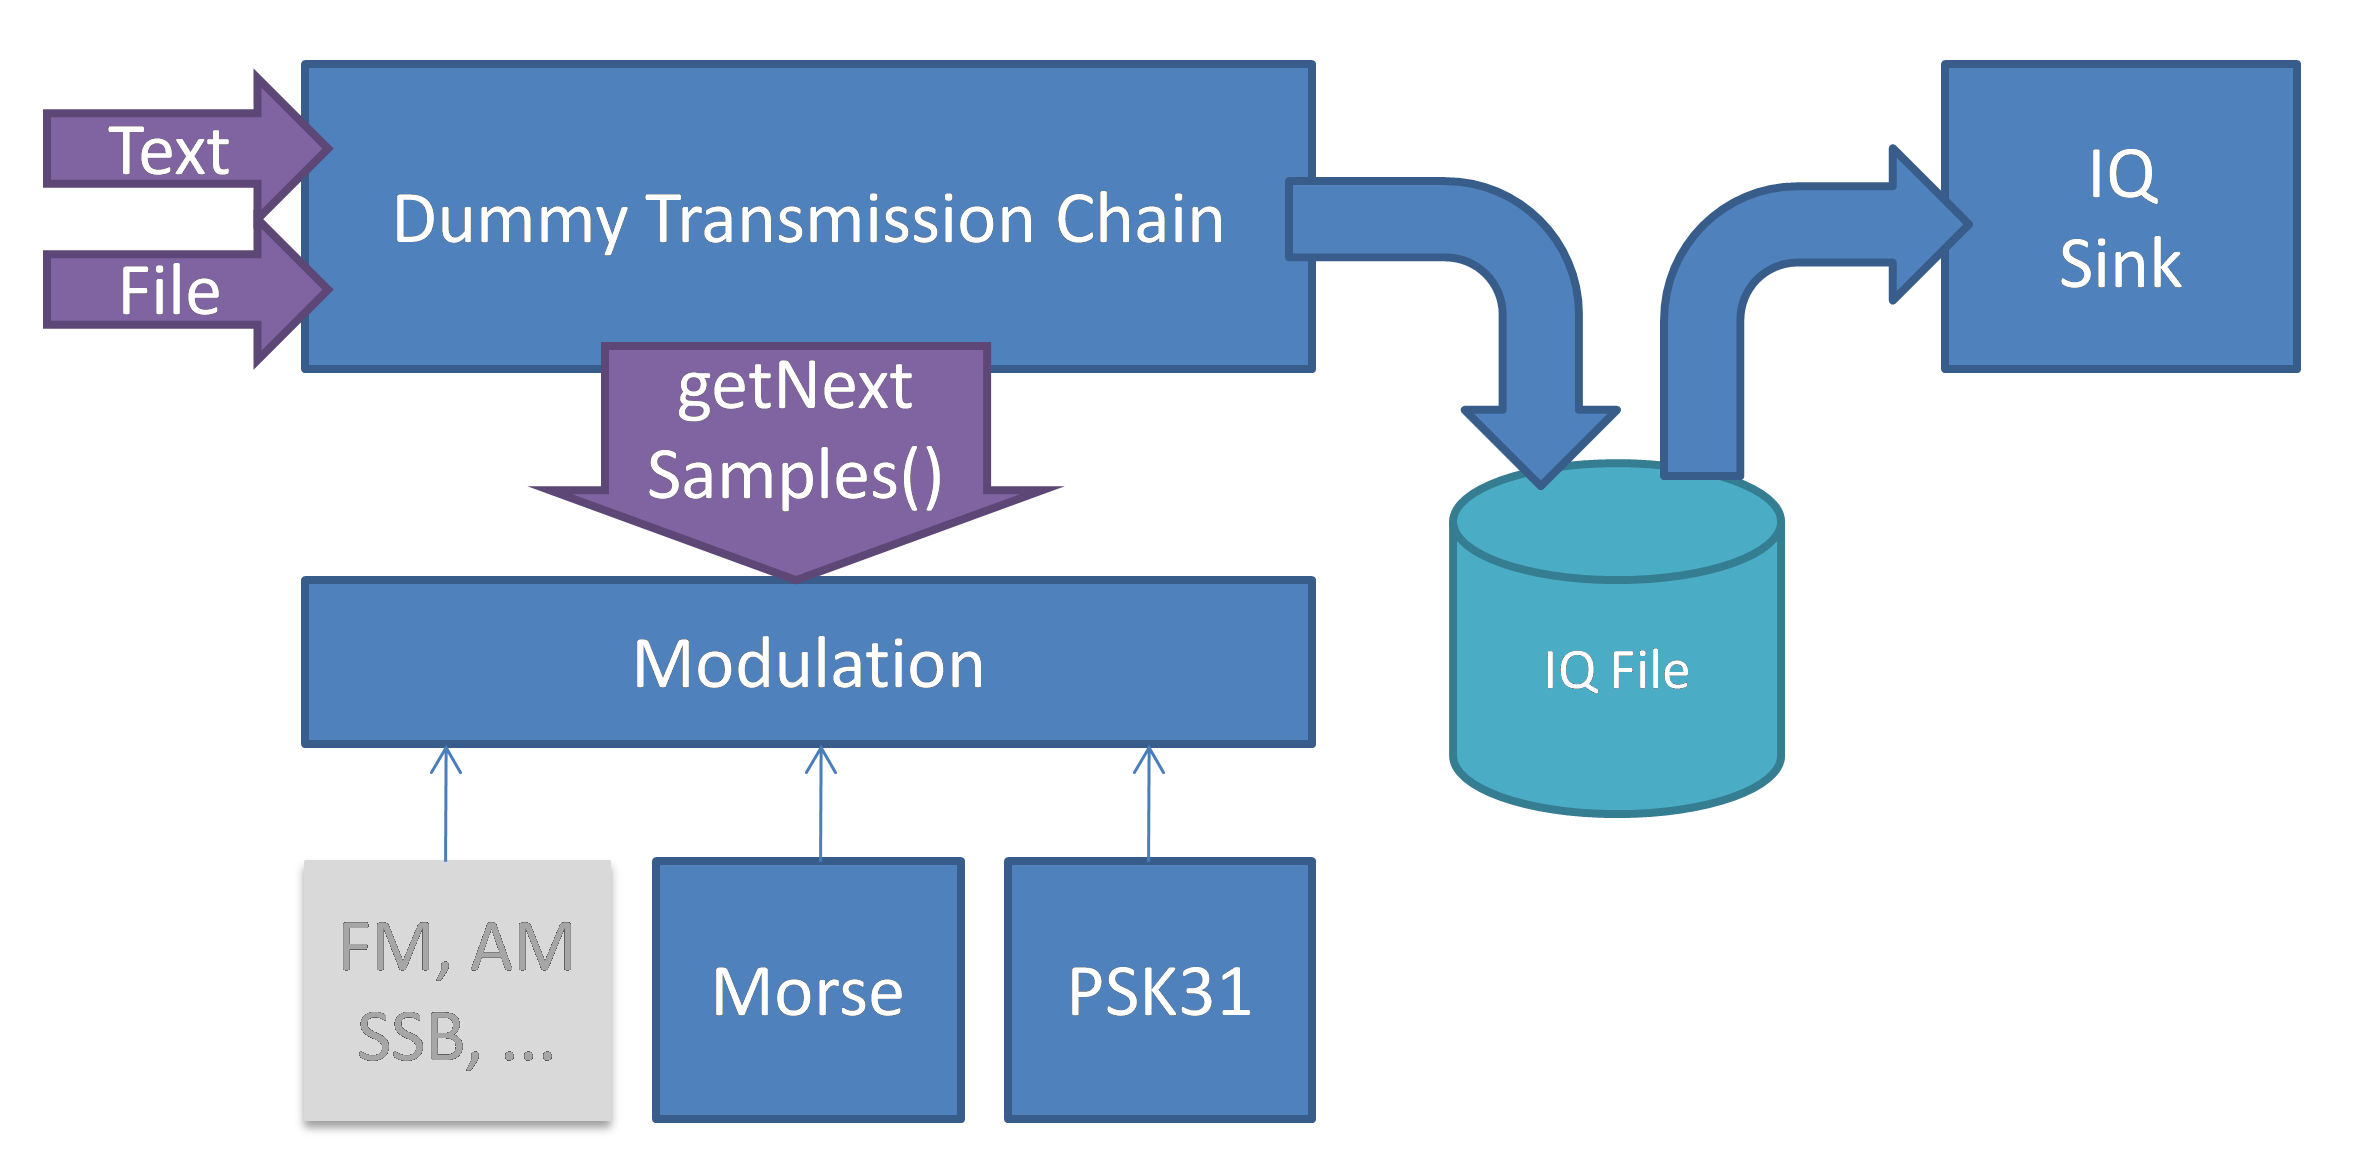
\includegraphics[width=1\linewidth]{gfx/TX_chain_step2.png}
	\caption{Transmission in current version of AnSiAn \cite{Mantz2016}}
	\label{fig:tx_chain_old}
\end{figure}

\begin{figure}
	\centering
	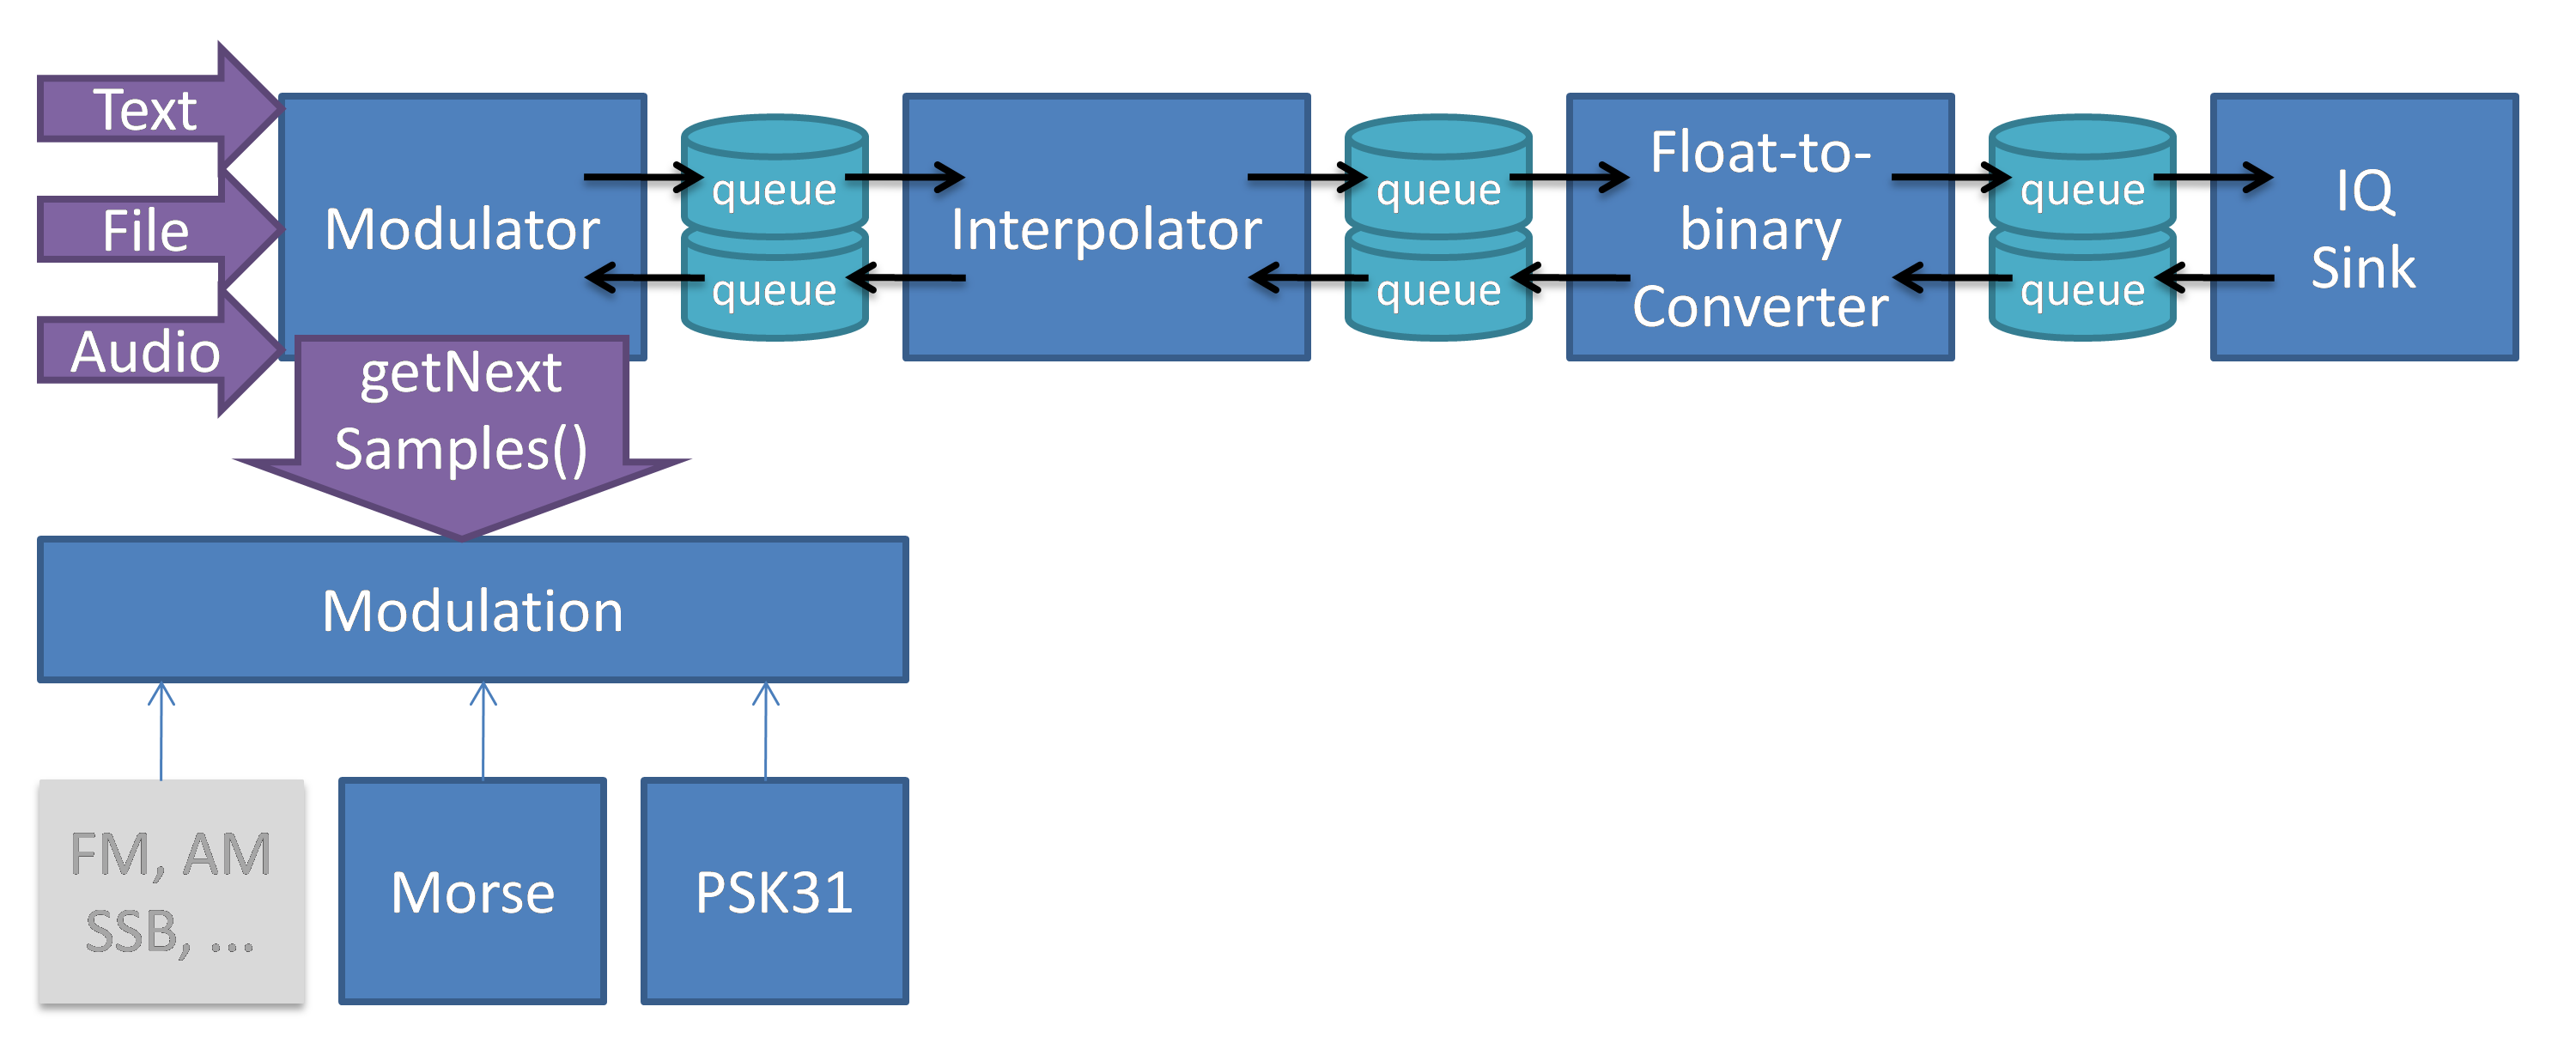
\includegraphics[width=1\linewidth]{gfx/TX_chain_final.png}
	\caption{Final transmission chain as suggested by \cite{Mantz2016}}
	\label{fig:tx_chain_new}
\end{figure}



\begin{figure}
	\centering
	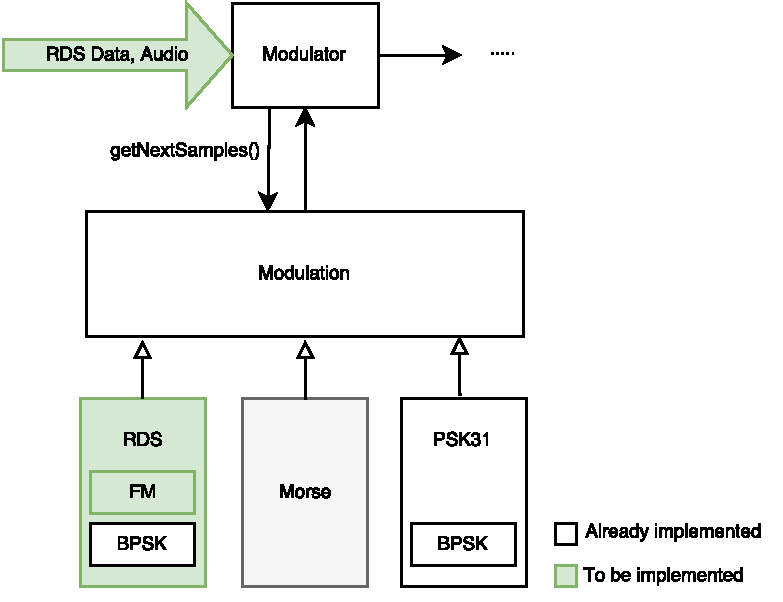
\includegraphics[width=1\linewidth]{gfx/feature2_components.pdf}
	\caption{Required Components for RDS Transmission}
	\label{fig:rds_transmission}
\end{figure}



\begin{figure}
	\centering
	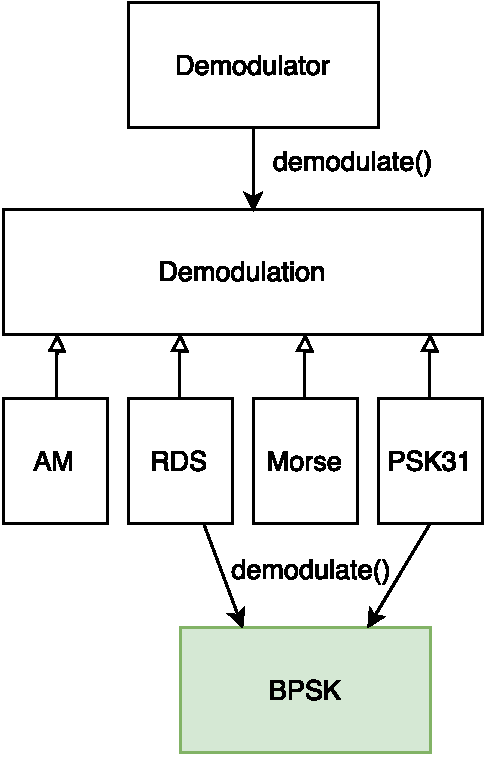
\includegraphics[width=0.5\linewidth]{gfx/feature3_components.pdf}
	\caption{Required Components for BPSK Demodulation Improvements}
	\label{fig:bpsk_components}
\end{figure}


\begin{figure}
	\centering
	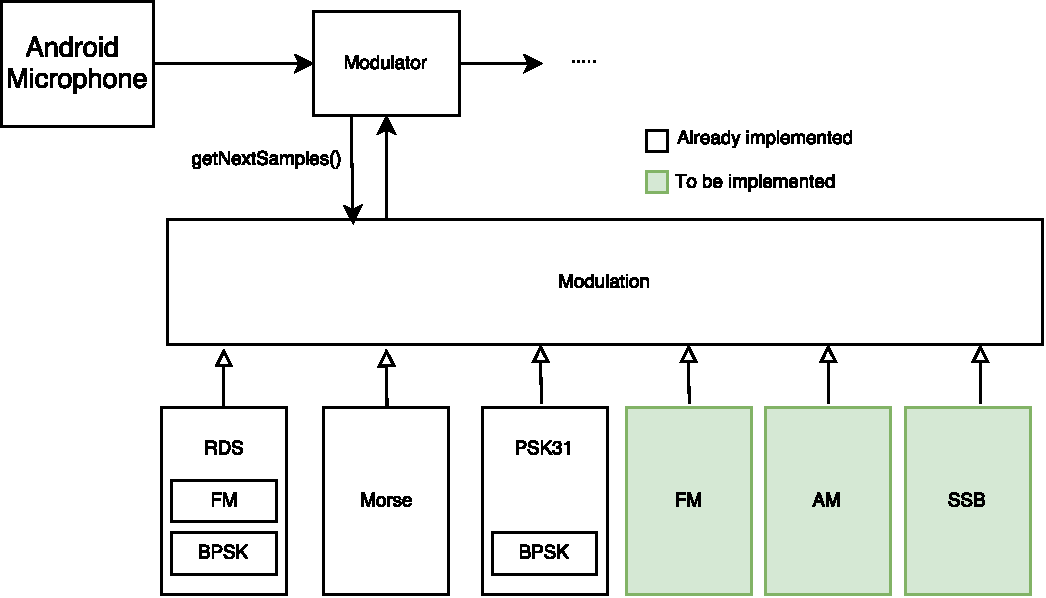
\includegraphics[width=1\linewidth]{gfx/feature4_components.pdf}
	\caption{Required Components for Walkie-Talkie-mode}
	\label{fig:walkie_talkie_components}
\end{figure}

% ********************************************************************
% Backmatter
%*******************************************************
\appendix
\cleardoublepage
%\ctparttext{The appendix contains some additional developments, that strongly supported us in the design of our communication system. Furthermore, it contains solutions to some problems.}
%\part{Appendix}
%\include{Parts/Part04}
%\include{Chapters/Part04_Chapter04_OOWARPLab}
%********************************************************************
% Other Stuff in the Back
%*******************************************************
\cleardoublepage%********************************************************************
% Bibliography
%*******************************************************
% work-around to have small caps also here in the headline
\manualmark
\markboth{\spacedlowsmallcaps{\bibname}}{\spacedlowsmallcaps{\bibname}} % work-around to have small caps also
%\phantomsection 
\refstepcounter{dummy}
\addtocontents{toc}{\protect\vspace{\beforebibskip}} % to have the bib a bit from the rest in the toc
\addcontentsline{toc}{chapter}{\tocEntry{\bibname}}
\label{app:bibliography}
\printbibliography
%\bibliography{Bibliography}
%\cleardoublepage\pagestyle{empty}

\hfill

\vfill


\pdfbookmark[0]{Colophon}{colophon}
\section*{Colophon}
This document was typeset using the typographical look-and-feel \texttt{classicthesis} developed by Andr\'e Miede. 
The style was inspired by Robert Bringhurst's seminal book on typography ``\emph{The Elements of Typographic Style}''. 
\texttt{classicthesis} is available for both \LaTeX\ and \mLyX: 
\begin{center}
\url{http://code.google.com/p/classicthesis/}
\end{center}
Happy users of \texttt{classicthesis} usually send a real postcard to the author, a collection of postcards received so far is featured here: 
\begin{center}
\url{http://postcards.miede.de/}
\end{center}
 
\bigskip

\noindent\finalVersionString

%Hermann Zapf's \emph{Palatino} and \emph{Euler} type faces (Type~1 PostScript fonts \emph{URW
%Palladio L} and \emph{FPL}) are used. The ``typewriter'' text is typeset in \emph{Bera Mono}, 
%originally developed by Bitstream, Inc. as ``Bitstream Vera''. (Type~1 PostScript fonts were made 
%available by Malte Rosenau and
%Ulrich Dirr.)

%\paragraph{note:} The custom size of the textblock was calculated
%using the directions given by Mr. Bringhurst (pages 26--29 and
%175/176). 10~pt Palatino needs  133.21~pt for the string
%``abcdefghijklmnopqrstuvwxyz''. This yields a good line length between
%24--26~pc (288--312~pt). Using a ``\emph{double square textblock}''
%with a 1:2 ratio this results in a textblock of 312:624~pt (which
%includes the headline in this design). A good alternative would be the
%``\emph{golden section textblock}'' with a ratio of 1:1.62, here
%312:505.44~pt. For comparison, \texttt{DIV9} of the \texttt{typearea}
%package results in a line length of 389~pt (32.4~pc), which is by far
%too long. However, this information will only be of interest for
%hardcore pseudo-typographers like me.%
%
%To make your own calculations, use the following commands and look up
%the corresponding lengths in the book:
%\begin{verbatim}
%    \settowidth{\abcd}{abcdefghijklmnopqrstuvwxyz}
%    \the\abcd\ % prints the value of the length
%\end{verbatim}
%Please see the file \texttt{classicthesis.sty} for some precalculated 
%values for Palatino and Minion.
%
%    \settowidth{\abcd}{abcdefghijklmnopqrstuvwxyz}
%    \the\abcd\ % prints the value of the length





\cleardoublepage% ******************************************************* Declaration
% *******************************************************
\refstepcounter{dummy}
%\pdfbookmark[0]{Thesis Statement}{statement} \chapter*{Thesis Statement}
\thispagestyle{empty}
\begingroup
%\let\cleardoublepage\relax
%\begin{flushright}
%	\emph{pursuant to §\,22 paragraph 7 of APB TU Darmstadt}
%\end{flushright}
%I herewith formally declare that I have written the submitted \myDegree{} independently. I did not use any outside support except for the quoted literature and other sources mentioned in the paper. I clearly marked and separately listed all of the literature and all of the other sources which I employed when producing this academic work, either literally or in content. This thesis has not been handed in or published before in the same or similar form.
%In the submitted thesis the written copies and the electronic version are identical in content.

%\bigskip

%\noindent\textit{\myLocation, \myTime}

%\smallskip

%\begin{flushright}
%	\begin{tabular}{m{5cm}}
%		\\ \hline
%		\centering\myName \\
%	\end{tabular}
%\end{flushright}

%\vfill

\selectlanguage{ngerman}
\pdfbookmark[0]{Erklärung}{erklaerung} \chapter*{Erklärung}
\begin{flushright}
	\emph{gemäß §\,22 Abs.\,7 APB der TU Darmstadt}
\end{flushright}
Hiermit versichere ich die vorliegende \myDegree{} ohne Hilfe Dritter und nur mit den angegebenen Quellen und Hilfsmitteln angefertigt zu haben. Alle Stellen, die Quellen entnommen wurden, sind als solche kenntlich gemacht worden. Diese Arbeit hat in gleicher oder ähnlicher Form noch keiner Prüfungsbehörde vorgelegen.
In der abgegebenen Arbeit stimmen die schriftliche und elektronische Fassung überein.

\bigskip
 
\noindent\textit{\myLocation, \myTime}

\smallskip

\begin{flushright}
    \begin{tabular}{m{5cm}}
        \\ \hline
        \centering\myName \\
    \end{tabular}
\end{flushright}

\selectlanguage{american}

% ********************************************************************
% Game Over: Restore, Restart, or Quit?
%*******************************************************
\end{document}
% ********************************************************************
